\section{Introduction}
%Medical devices operate across a range of invasiveness and intervention with the patient in the loop. For diagnostic-only devices, e.g. an X-ray machine, the physician operates the device to obtain patient data, perform diagnosis and deliver proper therapy to the patient (\figref{closed-loop}.(a)). For therapy-only devices, e.g. a drug infusion pump, the physician configures the device infrequently based on prior diagnosis of the patient so the device executes the therapy on the patient (\figref{closed-loop}.(b)). We denote these devices as \textbf{Open-loop Medical Devices} as there is no direct feedback between the patient and the device. 
\subsection{Medical Devices That Autonomously Interacts With the Patient}
Medical devices are developed to diagnose patient diseases and/or perform therapy to treat the diseases. 
For diagnose-only or therapy-only devices, the device operates under the supervision of professionally-trained physicians, who has the domain knowledge and responsible for performing the correct diagnosis and deliver accurate therapy. Thus the safety of the device is mostly determined by how accurately it provides information to the physicians and its faithful operation as instructed by the physicians. 
However, the dependance on the physicians means reduced freedom of the patients. As technology progresses there is a class of devices with both diagnostic and therapeutic functions, i.e. implantable cardiac devices to treat cardiac arrhythmia, deep brain stimulation devices to treat Parkinson's disease and artificial pancreas to treat Type 1 diabetes. These devices capture and diagnose the patient's physiological conditions from sensory data, and deliver therapy in response. These devices usually operate (semi-) autonomously with very little human intervention. While patients can enjoy better life style and receive timely therapy, malfunctions or inappropriate therapies from these autonomous devices cannot be corrected timely, which can cause serious adverse effects on patients' health. Therefore these devices are usually classified into the highest risk category and undergo the most stringent regulation. We denote them as \textbf{Closed-loop Medical Devices}. 
%\begin{figure}[t]
		%\centering
		%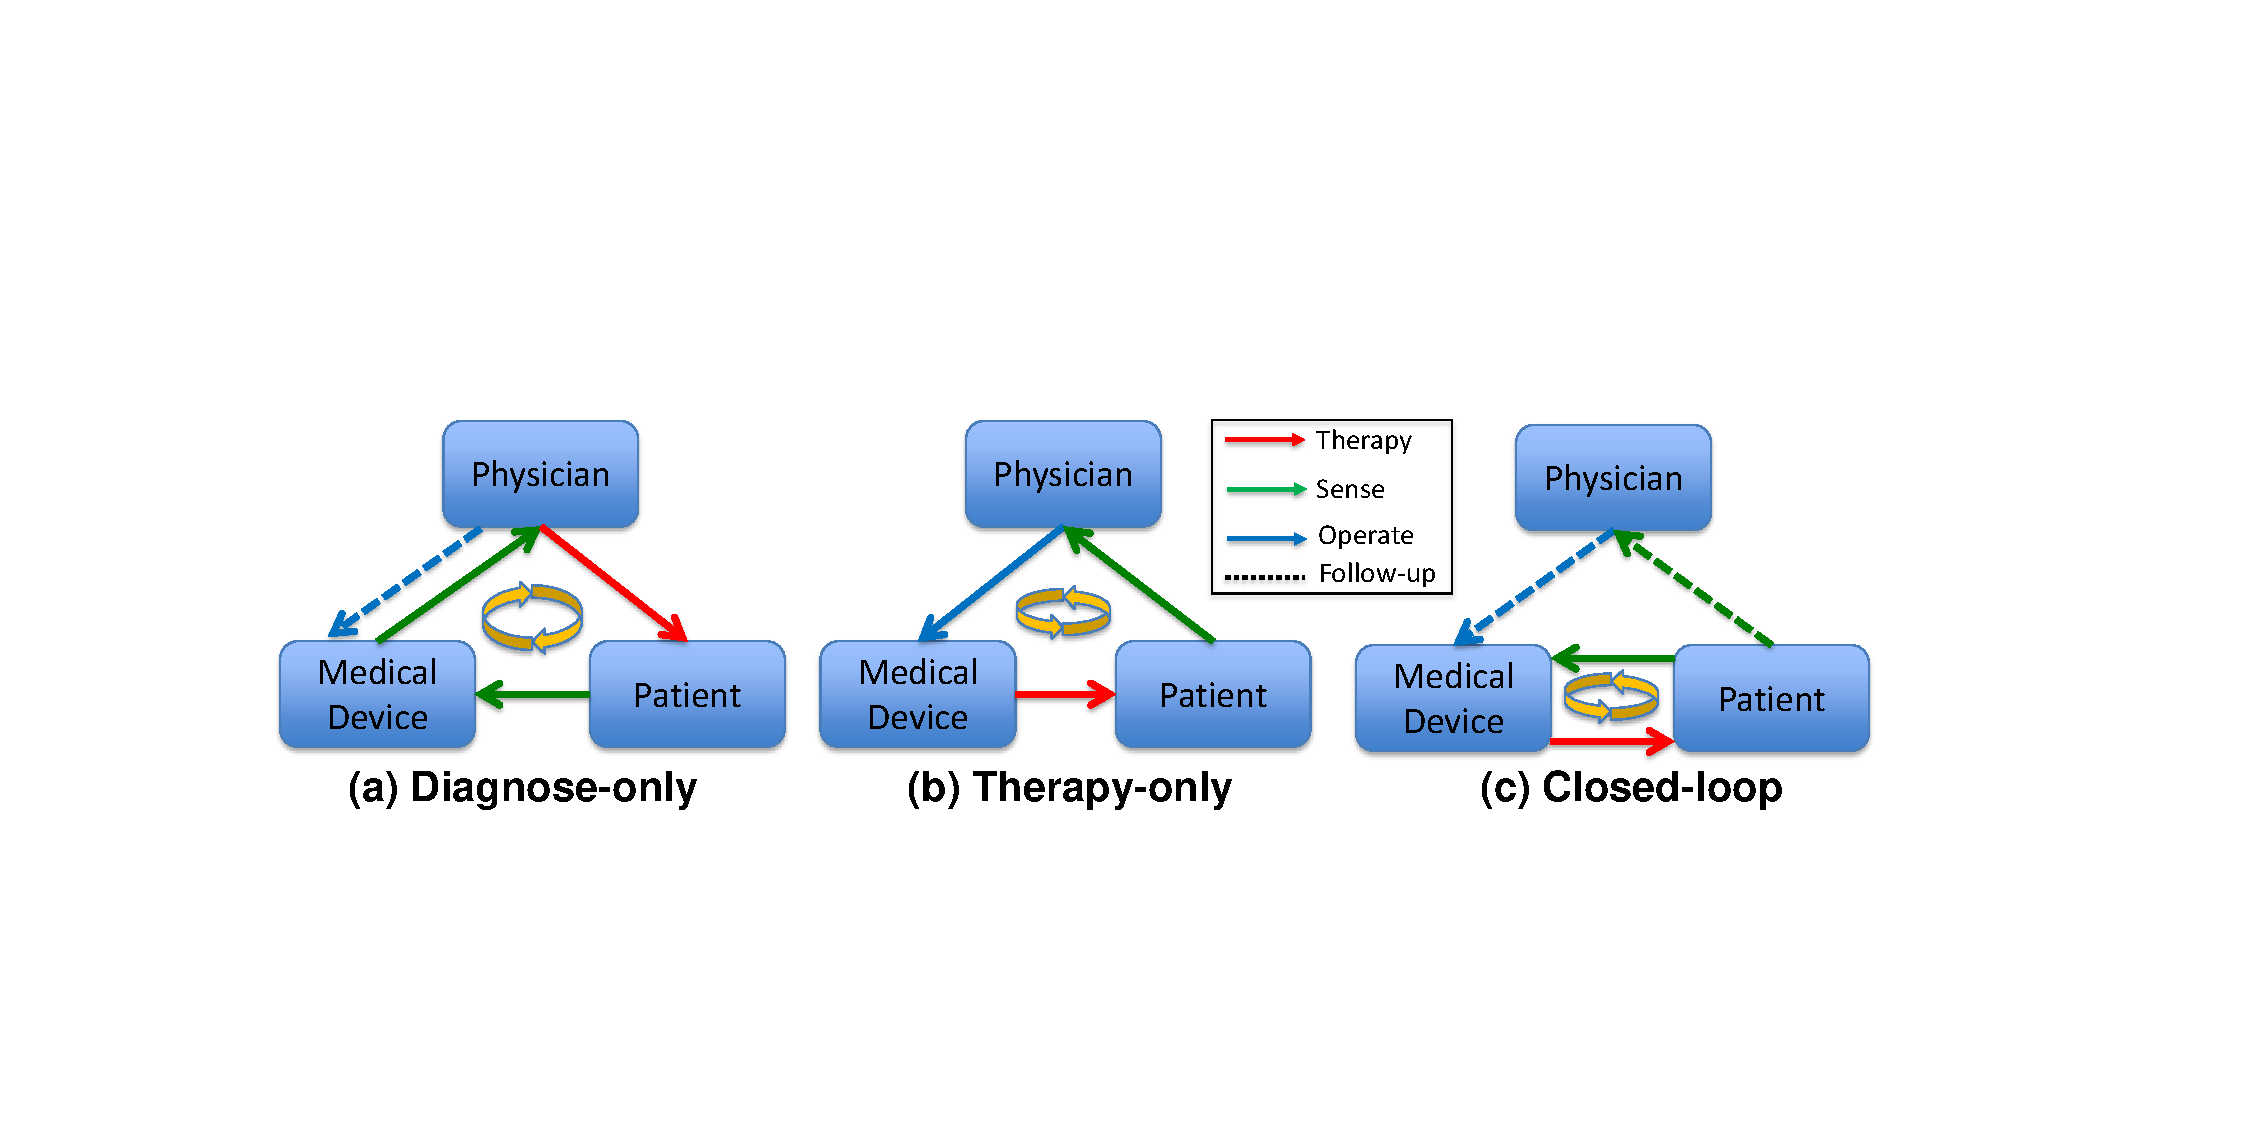
\includegraphics[width=\textwidth]{figs/closed-loop.pdf}
		%\caption{\small Diagnostic-only and therapy-only devices do not interact with the patient in direct closed-loop. The physician is responsible for the diagnostic and/or therapeutic decisions. However in closed-loop medical devices, the devices interact with the patient in closed-loop and have to make therapeutic decisions based on their own diagnosis.}
		%\label{fig:closed-loop}
%\end{figure}
Closed-loop medical devices pose significant challenges to the safety assurance process:\\
\textbf{Closed-loop Interactions with Complex Physiology: }\\
Closed-loop medical devices introduce new control loops into the patients' body, which may trigger adverse conditions through mechanisms which are unknown to both the developers and physicians. These mechanisms involve both the device and the patient, thus can only be identified when the device is working in its physiological environment.\\
%When using open-loop medical devices, the diagnosis and therapy decisions are made by medical professionals, who have expert knowledge of human physiology. Therefore they are able to identify adverse health conditions and adjust the therapy accordingly. On the other hand, closed-loop medical devices have to make both the diagnosis and therapy decisions on their own. The domain expertise required to make those decisions has to be programmed into the device. It is impossible to encode all the knowledge of human physiology into the device. Therefore, for unanticipated physiological conditions when the appropriate response has not been programmed into the device, the device may deliver inappropriate therapy which can cause adverse effect on patient's health. 
%Technological development of materials, sensors, embedded computing, energy storage, communications and packaging usher new closed-loop therapies (e.g. deep brain stimulation). While the spectrum of closed-loop interactions between the device and the human physiology may not be fully understood, the challenge is to ensure the device never drives the patient into an adverse state. Furthermore, even with well-understood behaviors, with the incremental addition of new therapies in legacy devices (e.g. cardiac rhythm therapy), may result in inadvertent and conflicted behavior ending up with inappropriate and unsafe operation. 
\textbf{Limited Diagnostic and Therapeutic Functions}\\
%One fundamental rationale behind closed-loop medical devices is to enable the patients to live their normal lives without the dependance of cumbersome medical devices and with minimal physician supervision. In fact, a large number of closed-loop medical devices are autonomous implantable devices. 
In order to minimize power consumption, heat dissipation and invasiveness, the sensing and therapy capabilities of the devices are limited. Limited sensing capabilities may cause misdiagnosis as the device may be unable to distinguish two sensed signals from different conditions that now seem similar and result inappropriate therapy. Due to limited therapeutic capabilities, there exists sub-optimal physiological conditions that are untreatable. \\
\textbf{Software-related Medical Device Recalls}\\
Due to the complexity of the diagnostic and therapeutic functions of the closed-loop devices, these functions are mostly controlled by their software components. 
%Software embedded in a medical device, unlike electrical and mechanical components, does not fail due to corrosion, fatigue or have statistical failures of subcomponents. Software failures are uniquely sourced in the design and development of the system. %Unlike other industries such as consumer electronics where product life cycles are measured in months, software engineering for medical devices often spans a decade and must prioritize safety and efficacy over time to market. 
%\begin{figure}[t]
		%\centering
		%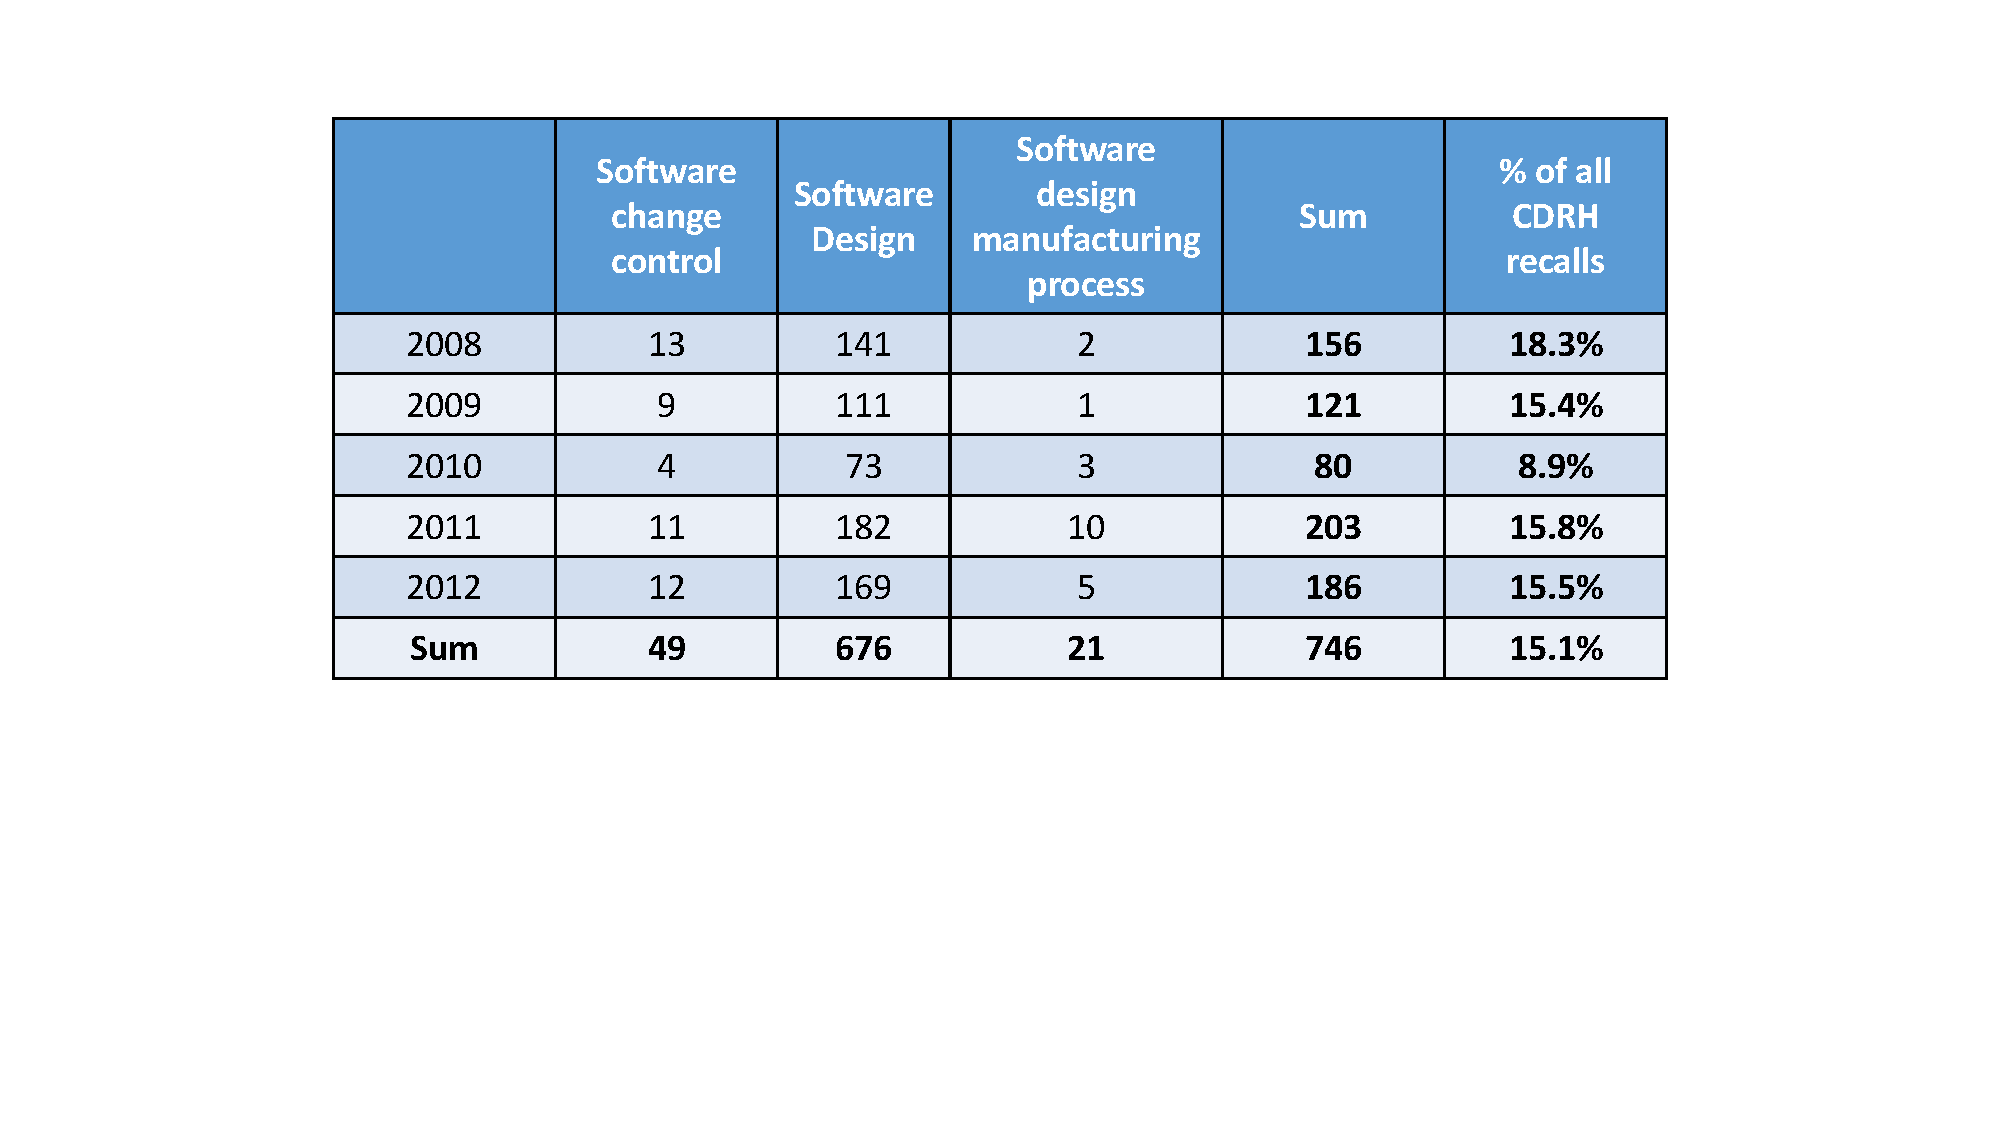
\includegraphics[width=0.8\textwidth]{figs/recalls.jpg}
		%\caption{\small Medical device recalls have risen over the past decade}
		%\label{fig:recalls}
%\end{figure}
%\begin{figure}[t]
		%\centering
		%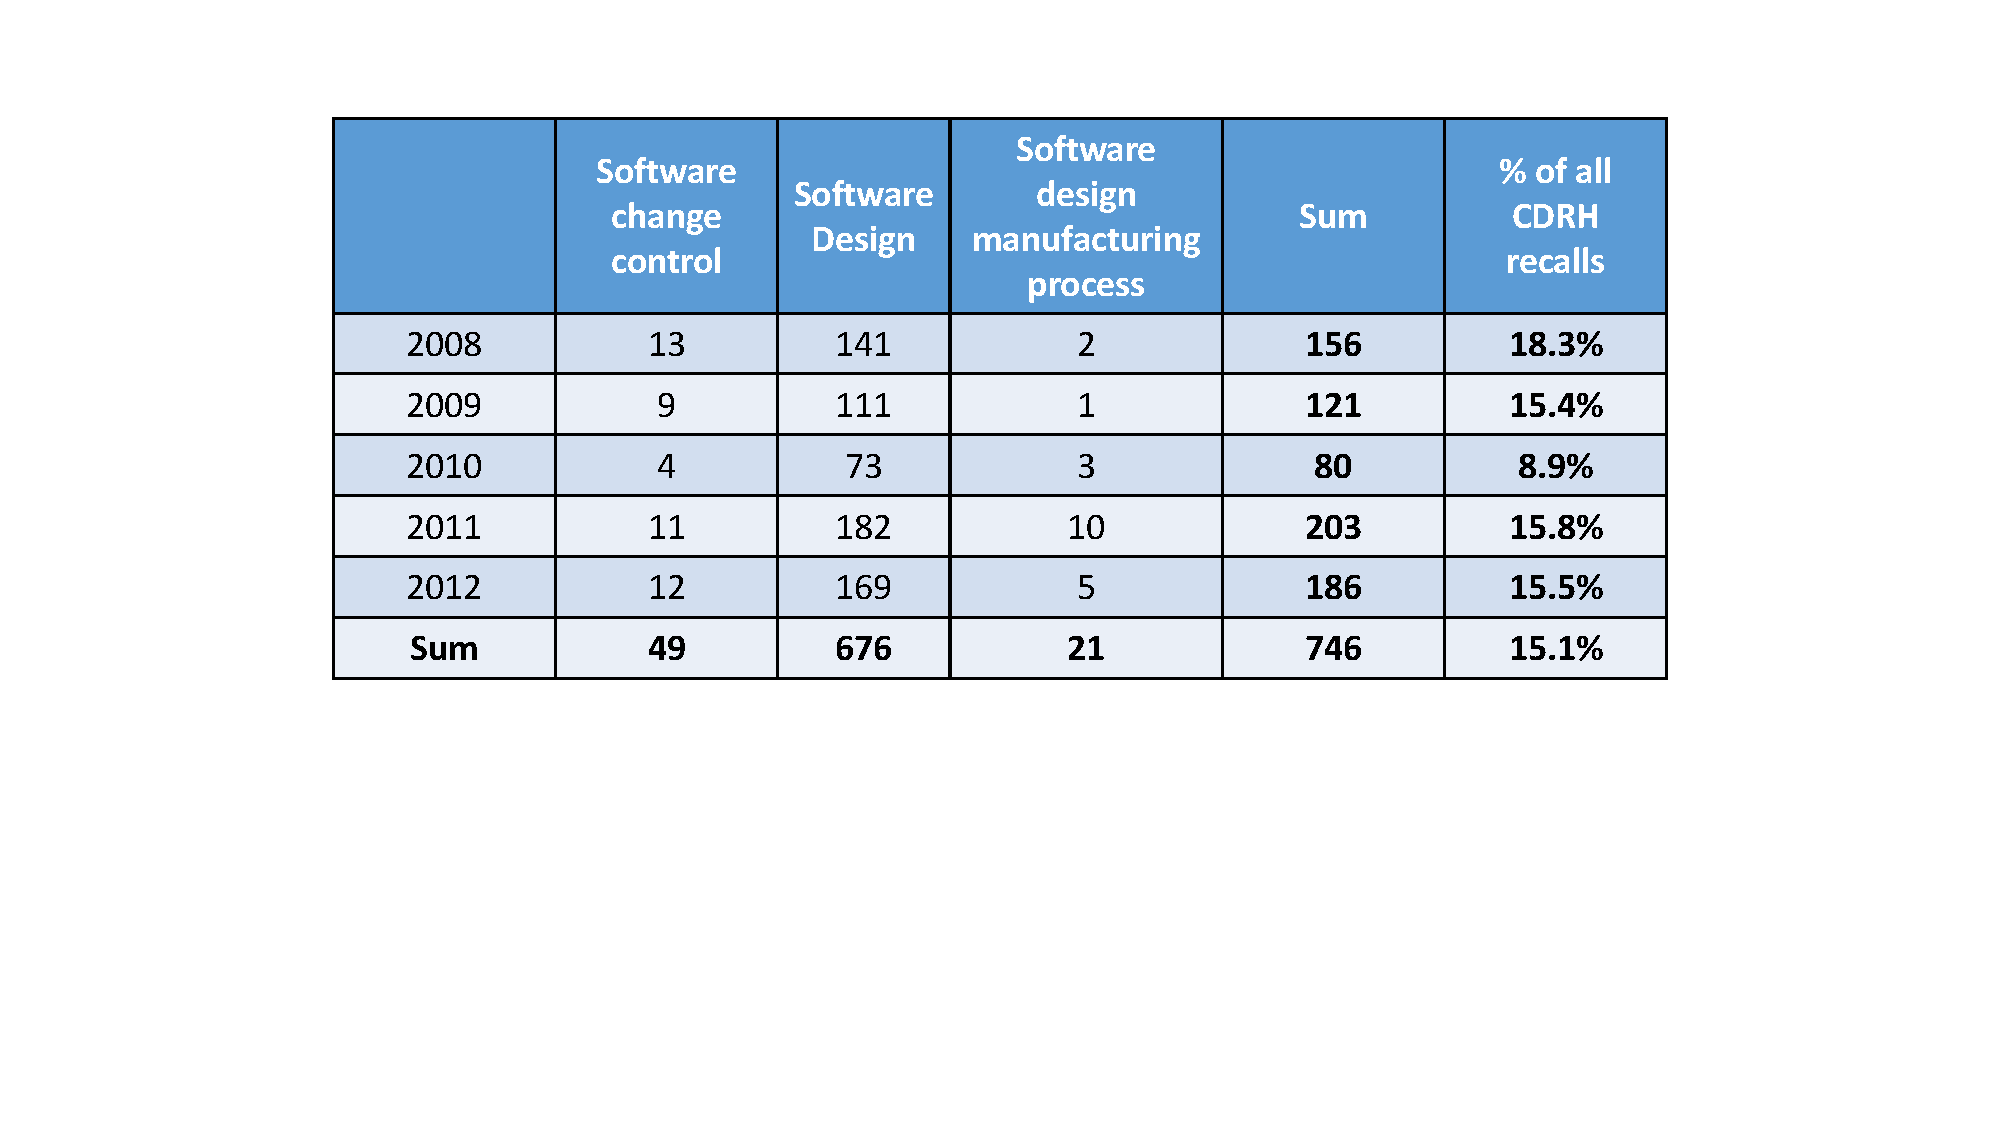
\includegraphics[width=0.8\textwidth]{figs/recalls.pdf}
		%\caption{\small Medical device recalls due to software issues have risen from 10\% in the 1990s to \~15\% in the past decade (\cite{recall_rep})}
		%\label{fig:soft_recalls}
%\end{figure}
%  Over the course of the past four decades, cardiac rhythm management devices such as pacemakers and implantable cardioverter defibrillators (ICD) have grown in complexity and now have more than 80,000 to 100,000 lines of code (\cite{pauljones}). 
According to the US Food and Drug Administration, in 1996, 10\% of all medical device recalls were caused by software-related issues. This percentage rose to an average of 15\% of recalls from 2008 to 2012. Malfunctions of closed-loop medical devices usually have severe consequences, which will be categorized as \emph{Class I}, meaning there is a ``reasonable probability that use of these products will cause serious adverse health consequences or death.'' 
\subsection{How to guarantee the safety of the medical devices?}
The medical device industry is regulated to ensure the safety of the patients and the public. In the United States, the FDA is the primary regulatory authority responsible for assuring the safety, efficacy and security of patients using medical devices. The device has to be \emph{validated} before entering the market, meaning there are sufficient evidence that the device is capable of fulfilling its \emph{intended purposes} without posing any danger to the patients.
%Based on the rationale that 1) manufacturers know their devices better than the regulator, and 2) the variety of medical devices requires a variety of approaches, it is the device manufacturers' responsibility to demonstrate the safety and efficacy of the medical devices. Manufacturers are required to complete a pre-market submission before the devices can be released to the market. The level of requirements for the submission is determined by the safety classification of the devices. 

Closed-loop medical devices have the highest safety classification, and have to be validated within its physiological context.
Clinical trials is the ultimate form of safety evidence for closed-loop validation.
Clinical trials have limitations
	

\subsection{How can physiological models help to improve medical device safety}
%With the deluge of software-based closed-loop medical devices in the coming years, relying on clinical trials as the only closed-loop evaluation method to identify risks is not scalable. Model-based design and virtual integration have been proposed and applied in other industries like automotive and avionics (\cite{autosar, avsi}), and can potentially help during the development process and provide extra confidence to the device before conducting clinical trials. However, unlike man-made systems like automobiles and aircrafts, physiological systems are less understood with larger variations. The lack of faithful models of physiological environment of the closed-loop medical devices is one of the reason that model-based design is not well-adopted in the medical device industry. 
As computational models of human physiology are developed, they can be used to interact with closed-loop medical devices or their models. The FDA is starting to recognize in silico modeling and simulation as regulatory-grade evidence for device safety and efficacy. For example, \cite{pancreas_paul} developed glucose-insulin models that can be used to evaluate control algorithms for artificial pancreas devices which can sense blood glucose and deliver insulin. Simulation results with the models have been recognized by FDA to replace animal trials, in part, which significantly reduced cost. With the increasing interest and recognition from the regulators, computer simulations are expected to play bigger role as safety and effectiveness evidence in the development of future closed-loop medical devices.

Physiological models developed for closed-loop evaluation of medical devices should have the following considerations:\\
\textbf{C1. Interfacing with the device: }The model should be able to generate physiological signals that the device sense from the real physiological entities. And the model should be able to take device output as input and change its states accordingly. \\
\textbf{C2. Differentiate different physiological conditions: }To evaluate the safety and effectiveness of the device, the device should be evaluated under specific physiological conditions. For example, the pacemaker is supposed to maintain proper heart rate during Bradycardia. The model should be complex enough to be able to differentiate the physiological condition (Bradycardia in the example) from other conditions. Failing to do so may result in false-positives or false-negatives in the evaluation result. \\
\textbf{C3. Physiological/logical interpretation of model states: } In closed-loop evaluation we are checking the device safety and effectiveness against the physiological requirements. However, due to the limited interface, it is always difficult to determine purely from an execution trace that the therapy is safe and effective. Therefore being able to provide physiological meanings to the states of the model also allows us to interpret the closed-loop execution more accurately, thus reduce the number of physiological-impossible executions during the evaluation. To satisfy these requirements, the model structure of these physiological models should base on physiological or clinical first principles so that states and state transitions of the closed-loop executions can be explained with physiological language. \\%One advantage of closed-loop evaluation over open-loop evaluation is the capability to provide physiological/logical interpretation of an execution trace. With this advantage we are able to identify and reduce the number of physiological-impossible executions by examining the state of the model, so that the evaluation can focus on physiological-possible executions. This requires the model first-principle\\
\textbf{C4. Available patient data: } In closed-loop evaluation, physiological models are developed to represent certain physiological condition or even a particular patient. The parameters of the model has to be identified so that the behaviors of the models match the behaviors of the patients (groups).  Due to the limited sensing capability of closed-loop medical devices, the data can be obtained are sparse. Therefore the complexity of the model should be in accordance with the available data to avoid \emph{over-fitting}, which occurs when a model having too many parameters relative to the number of observations and can introduce errors during prediction .

In this paper, we use implantable pacemaker and corresponding heart modeling as example, to demonstrate two applications of physiological modeling which provide safety evidence of closed-loop medical devices.
%We demonstrate two applications of closed-loop validation of closed-loop medical devices, using implantable pacemaker and corresponding heart modeling as example.
We focus on different modeling considerations and challenges for the two applications.

\begin{figure}[t]
		\centering
		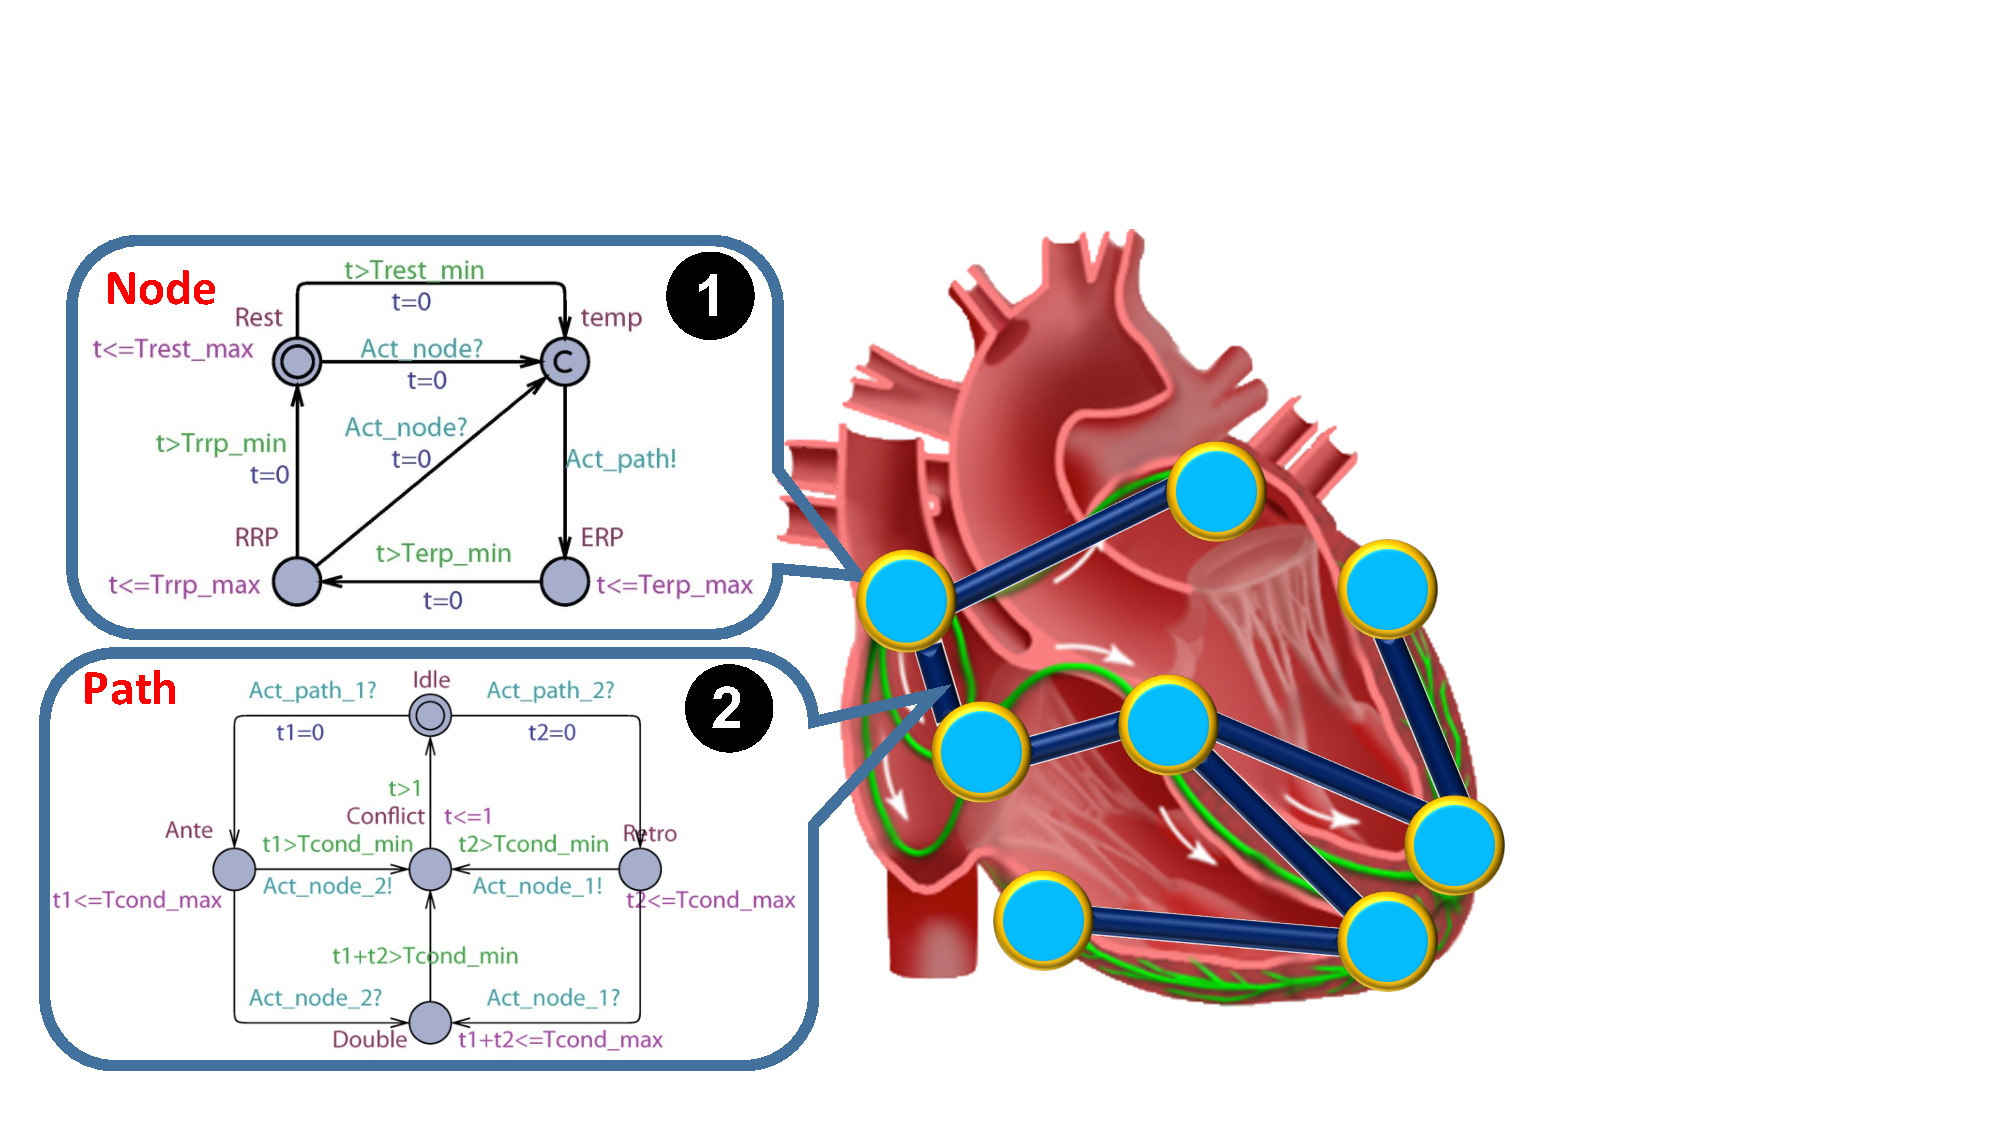
\includegraphics[width=\textwidth]{figs/Pacemaker.pdf}
		\caption{\small Percentage of computer simulation is expected to increase as safety and effectiveness evidence of medical devices}
		\label{fig:pacemaker}
\end{figure}
\section{How does the heart work and what are the models out there?}
The heart is the "motor" for blood circulation within our body. The heart has two ventricles which pumps the blood out of the heart, and two atria which gather blood from the body and pump them into the ventricles. 
The oxygen demand of the body changes during different activities. For example, the demand is higher while running and lower while sleeping. To satisfy these demands, the heart muscles in the atria and the ventricles have to contract with certain frequency and in accordance to optimize the \emph{Cardiac Output}, which refers to the volume of blood pumped by the heart per minute (mL blood/min). The coordinated contractions of the heart muscles are governed by the electrical conduction system of the heart (\figref{pacemaker}.(a)). 
A \emph{Normal Sinus Rhythm (NSR)} is the healthy heart rhythm which provides efficient blood flow. During a NSR, electrical signals are periodically generated by the \emph{Sinoatrial (SA) node} in the upper right atrium, which acts as the intrinsic pacemaker of the heart. The signals conduct throughout both atria and trigger muscle contractions to push blood into the ventricles. After a long conduction delay at the \emph{AV node} so that both ventricles are fully filled, the signals conduct through fast-conducting \emph{His-Purkinje} system to trigger almost simultaneous contractions of the ventricles and pump blood out of the ventricles. Derangement from NSR can result in insufficient cardiac output and thus insufficient oxygen supply to the body and/or the heart itself, which are referred to as \emph{Arrhythmia}. Arrhythmia impair the heart's ability to efficiently pump blood and compromise the patient's health. 
Arrhythmia are categorized into so-called \emph{Tachycardia} and \emph{Bradycardia}. Tachycardia features undesirable fast heart rate which can cause inefficient blood pumping. Bradycardia features slow heart rate which results in insufficient blood supply. Bradycardia are due to failure of impulse generation with anomalies in the SA node, or failure of impulse propagation where the conduction from atria to the ventricles is delayed or blocked. 
\subsection{First Principle Heart Modeling}
At cellular level, external electrical voltage can trigger ion channel activities of the heart muscle, causing it to contract. The ion channel activities change the external electrical voltage of the muscle which can trigger ion channel activities of the heart muscles nearby. This chain of activation is the basis for electrical signal conduction within the heart. Models for the cellular electrical activities have been developed to understand the relationship between ion channel activities and electrical and mechanical behaviors of heart tissue.

With development of imaging technologies like MRI, models of the heart anatomy can be obtained with very high resolution. These models contains detailed information of anatomical structures of the heart, i.e. fiber orientations, scar tissue after infarct. These detailed anatomy of the heart affect the behaviors of the heart thus anatomical models provides foundations for other whole heart modeling efforts. By combining the cellular models of the heart tissue and the detailed heart anatomy, models of the whole heart have been developed to study the mechanisms and mechanical effects of different arrhythmia. The models are also suitable for evaluating drug therapies that affects ion channel activities. Researchers from Johns Hopkins University also attempted to use electrical models combined with patient-specific anatomical model from MRI image to predict the onset of arrhythmia and evaluate their therapies.
\subsection{Behavior Models of Electrical Conduction}
Clinically, a common method to diagnose arrhythmia is using ElectroCardioGram (ECG), which are electrical signals of the heart measured on body surface. A more invasive but more accurate method is referred to as \emph{Electrophysiology (EP) testing}, in which physicians insert catheters with electrodes into the heart through the veins and local electrical activities around the electrodes can be measured. The \emph{patterns} of the electrical activities and the \emph{timing relationship} among them are used by the physicians to diagnose the heart conditions. The physicians can also obtain more information by manipulating the locations of the catheters and actively deliver electrical pacing through the catheters. The EP testing studies the timing properties of the generation and propagation of electrical signals through the electrical conduction system, and can accurately diagnose and even treat most arrhythmia. 

In \cite{VHM_proc}, researchers from University of Pennsylvania developed a heart model structure based on clinical EP testing. Timing properties of electrical signal generation and blocking are modeled by the \emph{node automata} and the conduction delay between node automata are modeled by \emph{path automata}. Different heart conditions can be constructed with a network of node and path automata with different topologies and parameter settings. The model structure focus on high-level timing behaviors of the electrical signals, and still maintain clinical-interpretable structures. EP testing is also very popular so that there are abundant patient data available for parameter tuning. The model structure has been used for closed-loop validation of implantable pacemakers. %Behaviors that affects the observable inputs to the pacemaker are the \emph{generation}, \emph{conduction} and \emph{block} of the electrical signals. The signal generation and block properties are captured by \emph{node automata} and the signal conduction property is captured by \emph{path automata}. The topology captures the structure of the electrical conduction system of the heart.


\section{Implantable Pacemaker For Treating Bradycardia}
The implantable cardiac pacemakers are rhythm management devices designed to treat bradycardia. A typical dual chamber pacemaker has two leads inserted into the heart through the veins which can measure the local electrical activity of the right atrium and right ventricle respectively (\figref{pacemaker}.(b)). According to the timing between sensed impulses, the pacemaker may deliver electrical pacing to the corresponding chamber to maintain proper heart rhythm.

The pacemaker is based on the EP testing principles in terms of both diagnosis and therapy. It only senses from two locations in the heart and only utilize the timing of the activation signals. The pacing signals are also very similar to any activation 
%Models have been developed from different perspectives and are applied in different applications:\\
%\textbf{Anatomical models:} With development of imaging technologies like MRI, anatomical models of the heart can be obtained with very high resolution. These models contains detailed information of anatomical structures of the heart, i.e. fiber orientations, scar tissue after infarct. These models provides foundations for other modeling efforts.\\
%\textbf{Understand the mechanisms of arrhythmia:} With the help of anatomical models, researchers construct heart models to understand how structural or timing changes can disrupt electrical and mechanical behaviors of the heart. These models utilize the anatomical models and each spatial component is assigned a cellular level model of the electrical and mechanical behaviors of heart tissue. These models allow researchers to interpret clinical scenarios and experiment new therapies.\\
%\textbf{Patient-specific arrhythmia prediction:} A large varieties of arrhythmia are caused by electrical signals circling around structurally anomalies of the heart, i.e. scar tissue. Scar tissue can be identified with MRI. By constructing an electrical heart model of the patient using the MRI data, researchers can have a better idea whether the scar tissue of a specific patient can cause arrhythmia, which is non-invasive compared to traditional diagnosis techniques.
%
%
%\subsection{Heart model that captures the timing behaviors of the heart}
%The pacemaker only measures electrical activities of the heart at two locations, and only uses the timing of the electrical events for diagnosis. Given the simple interface between the pacemaker and the heart, a heart model that captures the observable behaviors to the pacemaker is enough to generate inputs to the pacemaker. In \cite{VHM_proc} we developed a heart model structure based on clinical Electrophysiology testing. Behaviors that affects the observable inputs to the pacemaker are the \emph{generation}, \emph{conduction} and \emph{block} of the electrical signals. The signal generation and block properties are captured by \emph{node automata} and the signal conduction property is captured by \emph{path automata}. The topology captures the structure of the electrical conduction system of the heart.

%
%For different applications the model will have further considerations

\section{Explore all possible scenarios using model checking}
\subsection{What is model checking and what can it do?}
In semi-conductor industry, model checking and formal verification

Medical devices are designed to treat certain disease. But due to its closed-loop nature, the device has to be able to deal with the variability of the patient.

Hazard analysis
Can be used to identify unknown closed-loop mechanisms that may contribute to safety hazards.

%\subsection{Modeling the physiological environment for closed-loop model checking}
%Environment modeling considerations\\
%\textbf{Model Coverage: } While pacemakers are designed to treat bradycardia by maintaining the appropriate heart rate when the intrinsic rate is low. At the same time, a pacemaker should not adversely affect other heart conditions such as supraventricular tachycardia. Even for the same patient, the heart condition changes over time and must be covered by the model. In order to achieve safety across all possible heart conditions, the heart models used during closed-loop verification should be able to cover all possible heart behaviors, more precisely, their mapping to pacemaker inputs. Over-approximation with non-determinism can be used to simplify model structure while covering larger variety of environmental behaviors. Techniques like model-checking can then be used to examine the whole closed-loop state space for property violations.\\ 
%\textbf{Ambiguity Due To Low Sensing Capability: }The spatial sensing resolution of pacemakers is low, in terms of the number of sensing location (2-3 leads), as well as the information obtained from each sensing location (binary events). If abstraction rules utilize the fact that different heart conditions may generate exactly the same input sequence to the pacemaker, there will be ambiguities on concretizing abstract closed-loop executions. For certain conditional requirements, it is important to differentiate all possible concrete executions corresponding to an abstract execution. As the result, the heart model(s) should have the capability to differentiate these heart conditions when verifying certain properties.\\
%\textbf{Information Loss During Abstraction: }While over-approximation achieves simplicity and coverage, it also inevitably introduces invalid behaviors (e.g. not clinically feasible or relevant) into the model which can cause false-negatives and false-positives during model checking. To solve this problem, refined models of the heart should be available which can resolve spurious counterexamples and eliminate invalid executions when necessary to avoid false-positives.\\
%\textbf{Multi-level Abstractions:} Each requirement has different constraints on the environment conditions, which requires heart models at different abstraction levels. For example, "maintaining the heart rate above certain threshold" is a requirement that should be satisfied under all possible heart conditions. The appropriate heart model for this requirement should be able to cover inputs to the pacemaker under all possible heart conditions.
%
%\subsection{What is an example?}
\begin{itemize}
	\item ELT is a closed-loop condition (open vs. closed-loop)
	\item ELT was not discovered during development
	\item ELT is ambiguous to a healthy condition (require model refinement)
\end{itemize}
\begin{figure}[t]
		\centering
		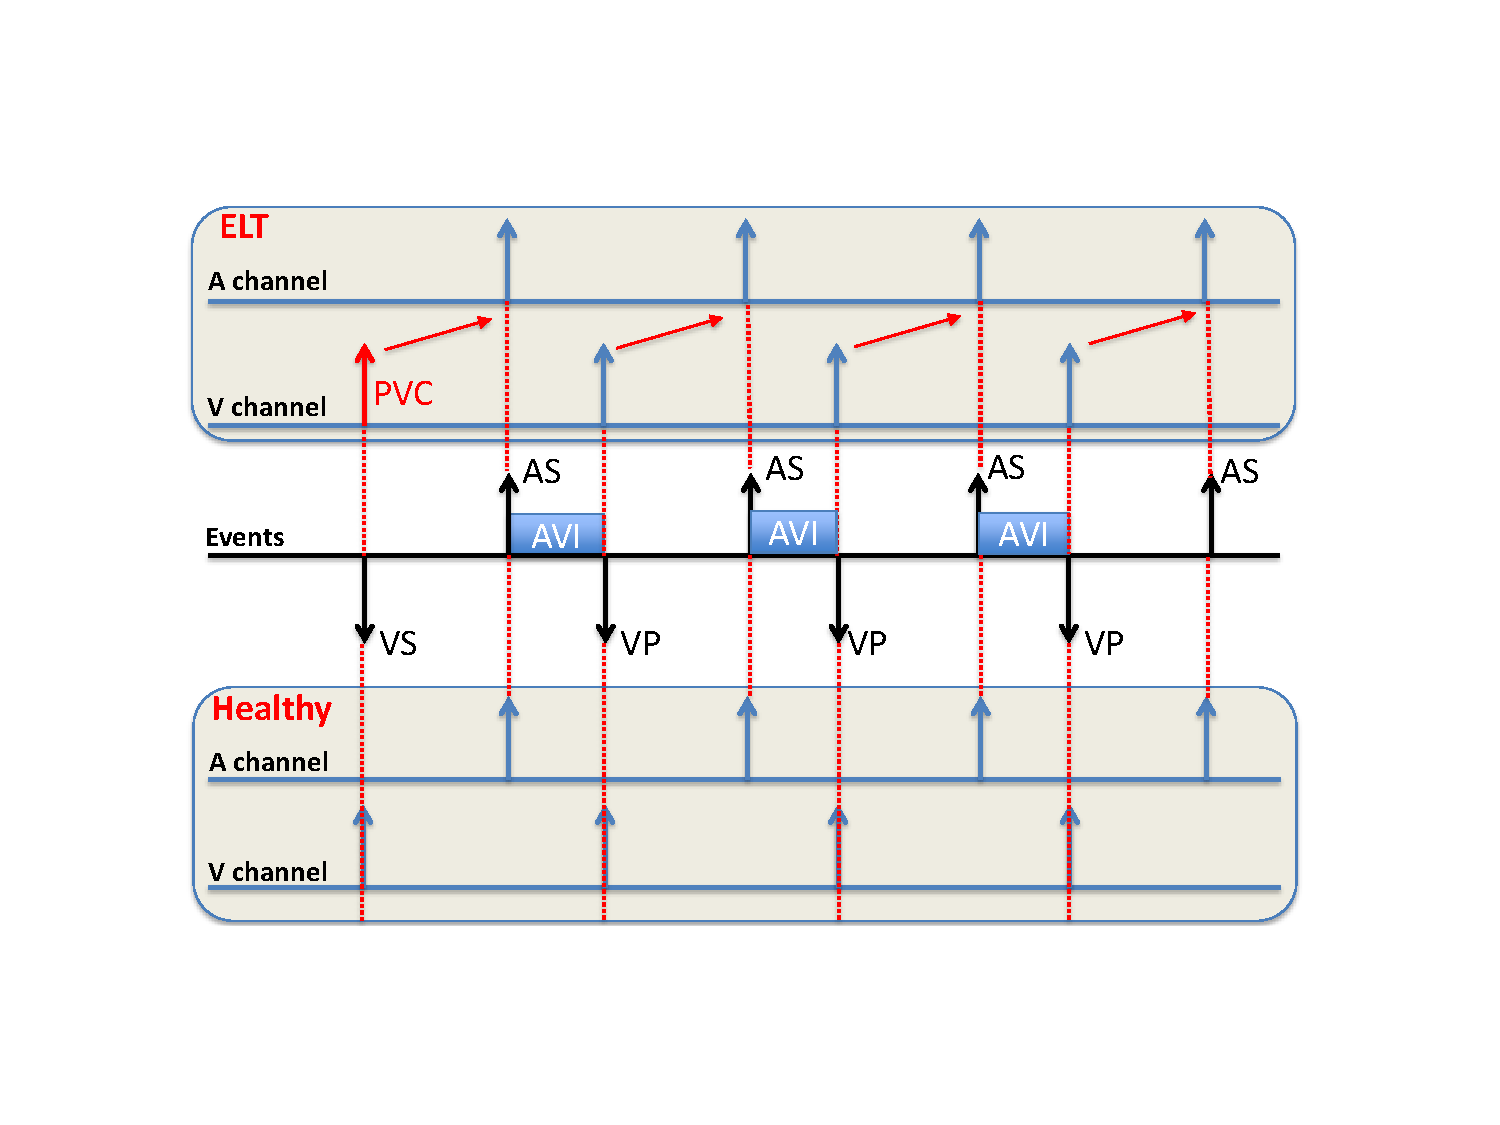
\includegraphics[width=\textwidth]{figs/ambiguity.pdf}
		\caption{\small Percentage of computer simulation is expected to increase as safety and effectiveness evidence of medical devices}
		\label{fig:ambiguity}
\end{figure}

